\documentclass[jou,apacite]{apa6}


\title{Hashtag Recommendation using Attention-based Convolutional Neural Network}
\shorttitle{APA style}
\newcommand\tab[1][1cm]{\hspace*{#1}}
\twoauthors{Bekirov Arthur, Dobrenkii Anton}{}
\twoaffiliations{University Innopolis}{}
\abstract{}

\usepackage{lipsum}
\usepackage{graphicx}

\usepackage{enumitem}
\rightheader{APA style}
\leftheader{Author One}

\begin{document}
\maketitle    




\section{Introduction}
Today microblogging services are used my millions of people, who use them for making short posts. The users also can include hashtags in their text. A hashtag is a string with a hash symbol in front of the words, commonly used for expressing the main idea of the text. With an enormous increase in microblogging services usage among social nets hashtags attract more attention as efficient tools for data mining such as public opinion analysis, microblog retrieval, prediction, etc. \\
The problem is, that there is a small number of posts with hashtags made by the authors. Thus and automated hashtag recomendation became an interesting area for research.\\

\section{Background}
Due to attention to this problem a big variety of methods were suggested. We can roughly divide them in collaborative filtering, generative and classification models. However, most of them are state-of-the-art solutions those are efficient on a specific task they were made for. According to ~\cite{Gong} we can use Convolutional Neural Network instead to increase the performance for hashtag recommendation. However, a standard CNN cannot operate with text, so authors propose an attention model for data integration.   \\ 
Before replicating ~\cite{Gong} experiment, we tested authors model on images as a solution for wrinkle detection task. There we discovered that the model can be enhanced with Gradient Boosting and, as a result, showing even better performance.


\section{Materials}
In the following work we used ~\cite{DBLP} dataset containing 50M user tweets as a test set. For training set based on word2vecapi a pretrained twitter dataset with 27B tweets (https://github.com/3Top/word2vec-api)  is used.


\section{Methods}
In this section our solution will be described in details. 
Consisting of the following parts:

\begin{enumerate}[itemsep=0mm]
    \item Enhancement scheme
    \item Data preprocessing
    \item Gradient boosting
    \item The results \\
\end{enumerate} 

\emph{\large{1. Enhancement scheme}}\\
Before we start describing our own solution, let's take a look on the model suggested in ~\cite{Gong}. Global and local channels combined are processed through the Softmax function. 
\begin{figure}
    \centering
    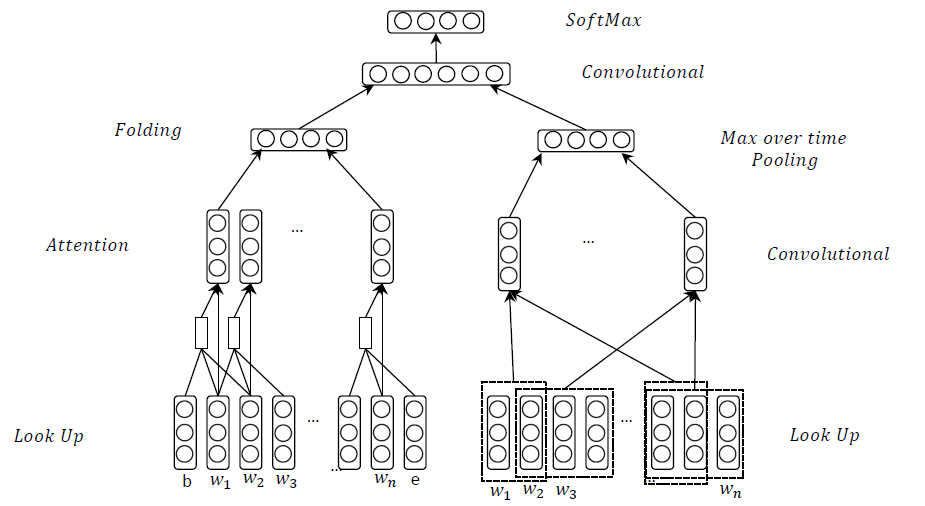
\includegraphics[scale=0.4]{Scheme.PNG}
    \caption{Initial attention-based Convolutional Neural Network}
    \label{fig:my_label}
\end{figure}

As the CNN processes run efficiently, we see that the result can be improved by additional data treatment before we begin analyzing it (dropout - ~\cite{Drop}) and after layers combination (Gradient Boosted Trees). \\

\begin{figure}
    \centering
    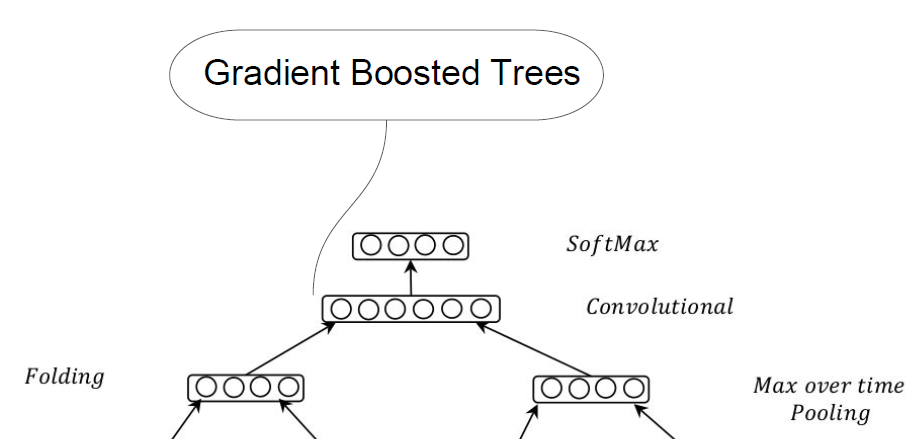
\includegraphics[scale=0.3]{123.PNG}
    \caption{Architecture enhancement}
    \label{fig:my_label}
\end{figure}

\emph{\large{2. Data preprocessing}}\\
Our initial dataset from ~\cite{DBLP} contained text, tweet, retweet count, URLs, mentioned entities. Thus it consisted of too much information which was odd for our research. What is more, not all the tweets had hashtags made by authors. So firstly we got rid of the odd data and collected 11 279 920 posts with hashtags.\\
However, the resulting dataset still cannot be processed by CNN. Our next step was text translation into vectors. As we had the pretrained twitter dataset we only had to look for the word in vocabulary. The resulting dataset consisted of strings with vectors and hashtags for final evaluation.\\
Although CNN is easier to train as it has fewer parameters, we still can effectively use dropout method suggested in ~\cite{Drop}. The key idea is to  randomly drop units (along with their connections) from the neural network during training. This prevents units from co-adapting too much, minimizes overftting and gives major improvements over other regularization methods.\\

\emph{\large{3. Gradient boosting}}\\
As the authors run the results of combined layers only through Softmax function, we suggest to apply GB-Trees with the help of DART booster ~\cite{Dart} As DART performs k-fold cross-validation (we take k = 5) we can estimate how accurately a predictive model will perform in practice.

\begin{figure}
    \centering
    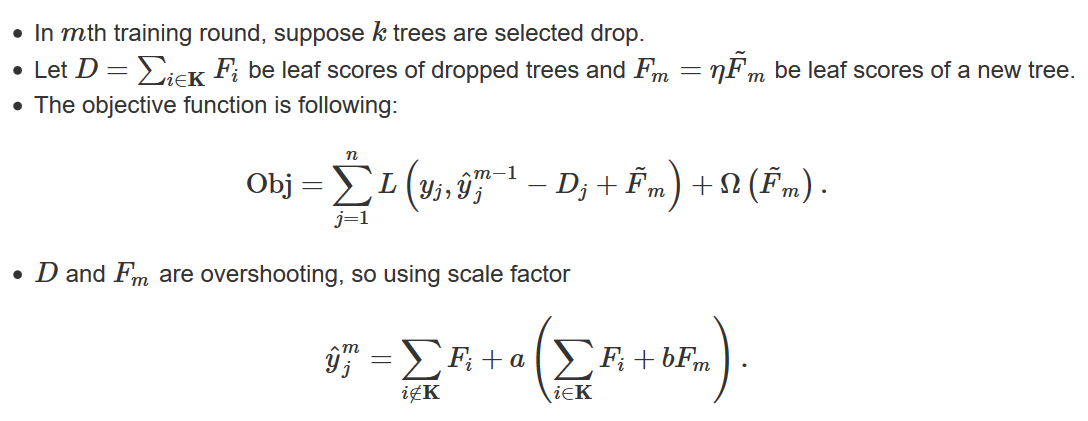
\includegraphics[scale=0.3]{dart.PNG}
    \caption{DART XGBoost algorithm}
    \label{fig:my_label}
\end{figure}
\emph{\large{4. The results}}\\
Upon applying the suggested method to images as a solution for wrinkle detection task we managed to outperform the authors model by 4\%. Model by ~\cite{Gong} showed $F_1$ score = 0.2 while our had $F_1$ score = 0.208 The inefficiency of scores itself can be explained as $F_1$ score can't be used properly for images, however we still managed to show better performance.\\ 
\begin{figure}
    \centering
    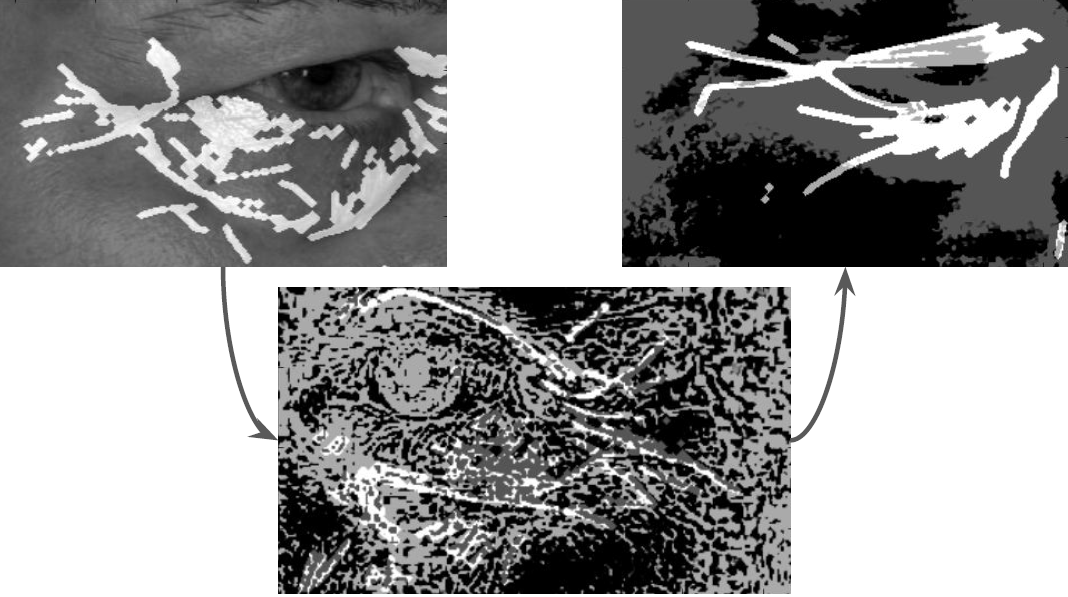
\includegraphics[scale=0.3]{eye.PNG}
    \caption{Wrinkle detection task}
    \label{fig:my_label}
\end{figure}
As for the text results, suggested architecture showed better prediction accuracy, however due to massive size of test set and  vocabulary we did not collect the evaluation results before the report submission. We are currently working on the collecting the scores and can update the outcome in the nearest future.\\



\bibliography{sample}

\end{document}
